\chapter{PID Controller Considerations}
\label{chap:PIDControllerConsideration}
\abstract{In this chapter the metrics used for performance and robustness evaluation are presented for the case of \gls{pid} control. Special attention is given to the integral measure of error.  Also the trade-offs that arises in a controlled system are considered, for example the well known relationship between servo and regulation response, or between performance and robustness. This trade-offs are what gives meaning to the multiobjective approach that will be presented in the rest of the book.}

\section{Control System Evaluation Metrics}
%
The need for quantitative metrics that provide insight in which measure a given controller tuning provides answer to a specific design criteria can be considered a common sense acceptable fact. However, it becomes an indispensable tool when coming to the need to combine different control system specifications, as it happens in a multiobjective approach.  It has been a common practice in the control systems literature to use different indexes to measure such properties accomplishment, both from the performance as well as robustness point of view.

Taking into account that in industrial process control applications, a good load-disturbance rejection as well as a good transient response to set-point changes is required, the controller design should consider both possibilities of operation. Despite this, the servo and regulation demands cannot be optimally satisfied simultaneously with a \gls{1dof} controller, because the resulting dynamic for each operation mode is different and it is possible to choose just one for an optimal solution. Therefore, there will be the need to quantify the level of \emph{performance} accomplishment regarding each one of the operational modes. On the other hand, the control system design is usually based on the use of low-order linear models; these models in turn are based on the normal operating point of the closed-loop control system. Because most industrial processes are non-linear, it is necessary to account for possible changes in the process characteristics by adopting certain relative stability margins or \emph{robustness} requirements for the control system.

Therefore, in the design of a closed-loop control system with PI and PID controllers, we must consider the trade-off between two conflicting criteria: the time-response performance to the set point and load disturbances and the robustness to changes in the characteristics of the controlled process. In order to manage those conflicting objectives in a suitable way, suitable metrics are presented in what follows.
 
\subsection{Performance}
%
The performance of a control system may be evaluated by using different measures. In control textbooks it is usual to find a characterisation of the time response in terms of numerical quantities assimilated to a second order underdamped system such as: percentage overshoot, rise time, etc. However, in academic and research works it is more usual and convenient to use a cost function based on the error, i.e. the difference between the desired value (set-point) and the actual value of the controlled variable (system's output).  Of course, as larger and longer in time is the error, the system's performance will be worse. In recent years have become very popular those related to the integrated error, given in general by the following formulation:
%
\begin{equation}
	J_{e} \doteq \int^{\infty}_{0} t^p \left|e(t)\right|^q dt,  \label{eq:generic_index}
\end{equation}
%
where the error can be generated because either of a set-point change or a load-disturbance.

A review of research history on \gls{pid} controller design reveals that, among the most used ones, there have been the \gls{iae}, the \gls{itae}, or the \gls{ise}. From an academic point of view, objective functions can take any one wished form. However, from an industrial point of view, realistic economic objectives need to be addressed. As it is desirable to use a performance indicator that takes into account economic considerations, the \gls{iae} is suggested \citet{Shinskey2002} as a meaningful measure as it can be assimilated to product giveaway, excess consumption of utilities, and reduction in plant capacity. Taking this into account, to avoid the cancellation of positive and negative errors, there seems to be a \emph{de facto} agreement with the use of the \gls{iae} ($p=0$, $q=1$ in \ref{eq:generic_index}) given by the following formula:
%
\begin{equation}
	J_e \doteq \int^{\infty}_{0} \left|e(t) \right| dt = \int^{\infty}_{0} \left|r(t)-y(t) \right| dt. 
\end{equation}
%
\subsection{Robustness}
%
Robustness is an important attribute for control systems, because the design procedures are usually based on the use of low-order linear models identified at the closed-loop operation point. Due to the non-linearity found in most of the industrial process, it is necessary to consider the expected changes in the process characteristics assuming certain relative stability margins, or robustness requirements, for the control system. The robustness is a measure of how much the controller can tolerate changes in the process transfer function; more specifically, in its gain and in its phase lag.

Also in this case there are some useful indicators that can be used as design criteria for robustness. The most widely accepted in industrial practice are the gain and phase margin. The \emph{gain margin $A_m$} is a measure of how much the process gain can change before the closed loop system becomes unstable. Control theory says it is the amount of gain increase or decrease required to make the loop gain unity at the frequency where the phase angle is $-180^o$. Therefore leading the closed-loop system to the critical point. On the other hand, the \emph{phase margin $\phi_m$} is a measure of how much the process phase can change before the closed loop system become unstable. The phase could be increased because of an additional delay or because the process lag decrease.

The use of the gain and phase margins as robustness measures, has been replaced by the use of a single indicator, the maximum of the sensitivity function, denoted by $M_s$, given by the shortest distance from the Nyquist diagram to the real point -1; this maximum sensitivity is strictly related to the gain and phase margin through some simple inequalities. Then, for each controller parameter set obtained, the closed-loop control system robustness is measured using control system Maximum Sensitivity $M_s$ defined as:
%
\begin{equation}
M_{s} \dot{=} \max_{\omega} \left|S(j \omega)\right| = \max_{\omega} \frac{1}{\left|1+C(j \omega) P(j \omega)\right|}
\label{Eq:Ms}
\end{equation}

The recommended values for $M_s$ are typically within the range 1.4 - 2.0 (\cite{astromhagglund2006}). The use of  the maximum sensitivity as a robustness measure, has the advantage that lower bounds to the gain, $A_m$, and phase, $\phi_m$, margins (\cite{astromhagglund2006}) can be assured according to
%
\begin{eqnarray*}
    A_m > \frac{M_s}{M_s-1} \quad ; \quad \phi_m > 2 \sin^{-1} \left(\frac{1}{2 M_s} \right)
\end{eqnarray*}

Therefore, ensuring $M_s=2.0$ provides what is commonly considered minimum robustness requirement (that translates to $A_m> 2$ and $\phi_m > 29^o$, for $M_s=1.4$  we have $A_m > 3.5$ and $\phi_m > 41^o$). Even if there are different measures for the closed-loop system robustness, the idea spread today to a common use of the maximum of the sensitivity function (commonly called $M_S$) as a reasonable robustness measure.
%
%\centerline{\textcolor{red}{TAKE A LOOK AT THE MODULUS MARGIN}}
%
\subsection{Control Input Usage}
%
Controller design problems are stated in terms of the controlled variable (usually the process output). Depending on how this problem is stated and solved, this may generate controller settings that produce command signals that are either undesirable or not realistic. It is therefore always needed to evaluate the control signal and take care of the controller bandwidth. This is usually related to the variation of the control signal as a measure of its \emph{smoothness}. For the evaluation of the required \emph{control effort} the control signal total variation $TV_u$ given by the difference between the values of the control variable at two consecutive sampling time instants:
%
\begin{equation}
	TV_u \doteq \sum^{\infty}_{k=1} \left|u_{k+1} - u_k \right|,  \label{eq:p02}
\end{equation}
%
is used as main indication of the smoothness of the control action for input changes.

As a complementary measurements of the control effort it can also be considered the controller output instant change to a set-point step change (the ``proportional kick'') given by
\begin{equation}
	\Delta u_0 \doteq \beta K_p \Delta r, \label{eq:p02du}
\end{equation}

\section{Control System Tradeoffs}
%
When considering a control task, there are different aspects the operator desires the control system to behave in a prescribed way or, why not, as better as possible. This is what we refer to control system performance with respect to, for example, set-point tracking, disturbance rejection, control effort reduction, and implicitly, with some degree of tolerance to a change in the process operating conditions: robustness. It is well known these goals are in conflict among them and cannot be achieved simultaneously \cite{Arrieta2010,alcantara2013} . In such case a trade-off between the objectives is required. Improving one objective may mean poor performance in another, or less robustness. As we have seen, every goal should be translated into design specifications, and specific indices in order to  measure the performance of the \gls{pid} controller.

Taking into account that in industrial process control applications, it is required a good load-disturbance rejection, as well as, a good transient response to set-point changes, the controller design should consider both possibilities of operation. Despite the above, the servo and regulation demands cannot be optimally satisfied simultaneously with a \gls{1dof} controller, because the resulting dynamic for each operation mode is different and it is possible to choose just one for an optimal solution. Considering the previous statement, most of the existing studies have focused only in fulfilling one of the two requirements, providing tuning methods that are optimal to servo-control or to regulation-control. However, it is well known that if we optimise the closed-loop transfer function for a step-response specification, the performance with respect to load-disturbance attenuation can be very poor and vice-versa \cite{Arrieta2010a}. Therefore it is desirable to get a compromise design, between servo/regulation when using \gls{1dof} controller.

Tuning is usually a compromise between performance and robustness. In fact, information about the process to be controlled takes the form of a model but this is always incomplete. Therefore, robustness is needed in order to preserve the basic properties that the model-based tuning provides. Among them, stability of the controlled system is a first need. Also, to minimise the degradation of the performance is desirable. As a basic tradeoff, as more robustness is imposed, the model-based tuning tends to provide lower performance. This is why some tunings focuses exclusively on loop performance, whereas others are aimed to ensure robust stability, or a compromised mix of both, etc. 

\subsection{Servo vs. Regulation}
%
When tuning standard \gls{pid} controllers, it is hard to achieve good tracking and fast disturbance rejection at the same time. From a specific tuning, if we want to improve disturbance rejection and get it faster, this requires more gain inside the bandwidth, which can only be achieved by increasing the slope near the crossover frequency. As a larger slope means getting closer to the critical (-1, 0j) point, this typically comes at the expense of more overshoot in response to set-point changes. Therefore worsening the set-point tracking. This is a frequency domain reasoning that is sometimes not familiar. Therefore, the use of time domain indexes like the ones presented above. A relatively low \gls{iae} corresponds to a relatively fast closed loop response and relatively low oscillatory behaviour in the controlled variable (also represented by low values in the control effort measure). 
 
As we already know, the closed loop transfer function between the set-point and error is different from that of the load disturbance and error; therefore a low \gls{iae} in fast tracking task leads to slow-moving behaviour with high \gls{iae} in the load disturbance rejection; conversely, a quick reaction to the disturbance means high overshoot in response to set-point step change, therefore increasing its \gls{iae}. This is a well known effect when zero-pole cancellation occurs in the closed loop transfer function. A solution usually taken for set-point tunings. It uses to work well for the operation as a servo control system but as the closed-loop relation from the load disturbance to the error still contains the process modes. Therefore explaining the regulation operation does not need to exhibit good performance measures.
 
It is usual practice, for \gls{1dof} controllers, to relate the tuning method to the expected operation mode for the control system, \emph{servo} or \emph{regulation}. Therefore, controller settings can be found for optimal set-point or load-disturbance responses. This fact allows better performance of the controller when the control system operates on the selected tuned mode but, a degradation in the performance is expected when the tuning and operation modes are different. Obviously there is always the need to choose one of the two possible ways to tune the controller, for set-point tracking or load-disturbances rejection. In the case of \gls{1dof} \gls{pid}, tuning can be optimal just for one of the two operation modes.

In order to show how the performance of a system can be degraded when the controller is not operating according to the tuned mode, an example is provided. This motivates the analysis of the servo/regulation \emph{trade-off}.

Consider the following plant transfer function, taken from \citet{zhuang1993}, and the corresponding \gls{foptd} approximation 
%
\begin{equation}
P_1(s)=\frac{\me^{-0.5s}}{(s+1)^2} \approx \frac{\me^{-0.99s}}{1+1.65s}. \label{system_example} 
\end{equation}

\gls{pid} controller parameters are found in \citet{zhuang1993} by application of the \gls{ise} tuning formulae for optimal set-point and load-disturbance. Figure \ref{ch3:fig:example1} shows the performance of both settings when the control system is operating in both, servo and regulation mode. It can be appreciated that the load-disturbance response of the set-point tuning ($sp$) is closer to the optimal regulation one than the load-disturbance tuning ($ld$) to the optimal servo tuning. Therefore the observed Performance Degradation is larger for the load-disturbance tuning. It is needed to search for a compromise among both tunings. If just one has to be taken, then it seems better to choose the set-point settings. However, as conflicting objectives, a more complex approach is needed in order find the best tradeoff (whatever best means).
%
\begin{figure}[tb]
    \begin{center}
        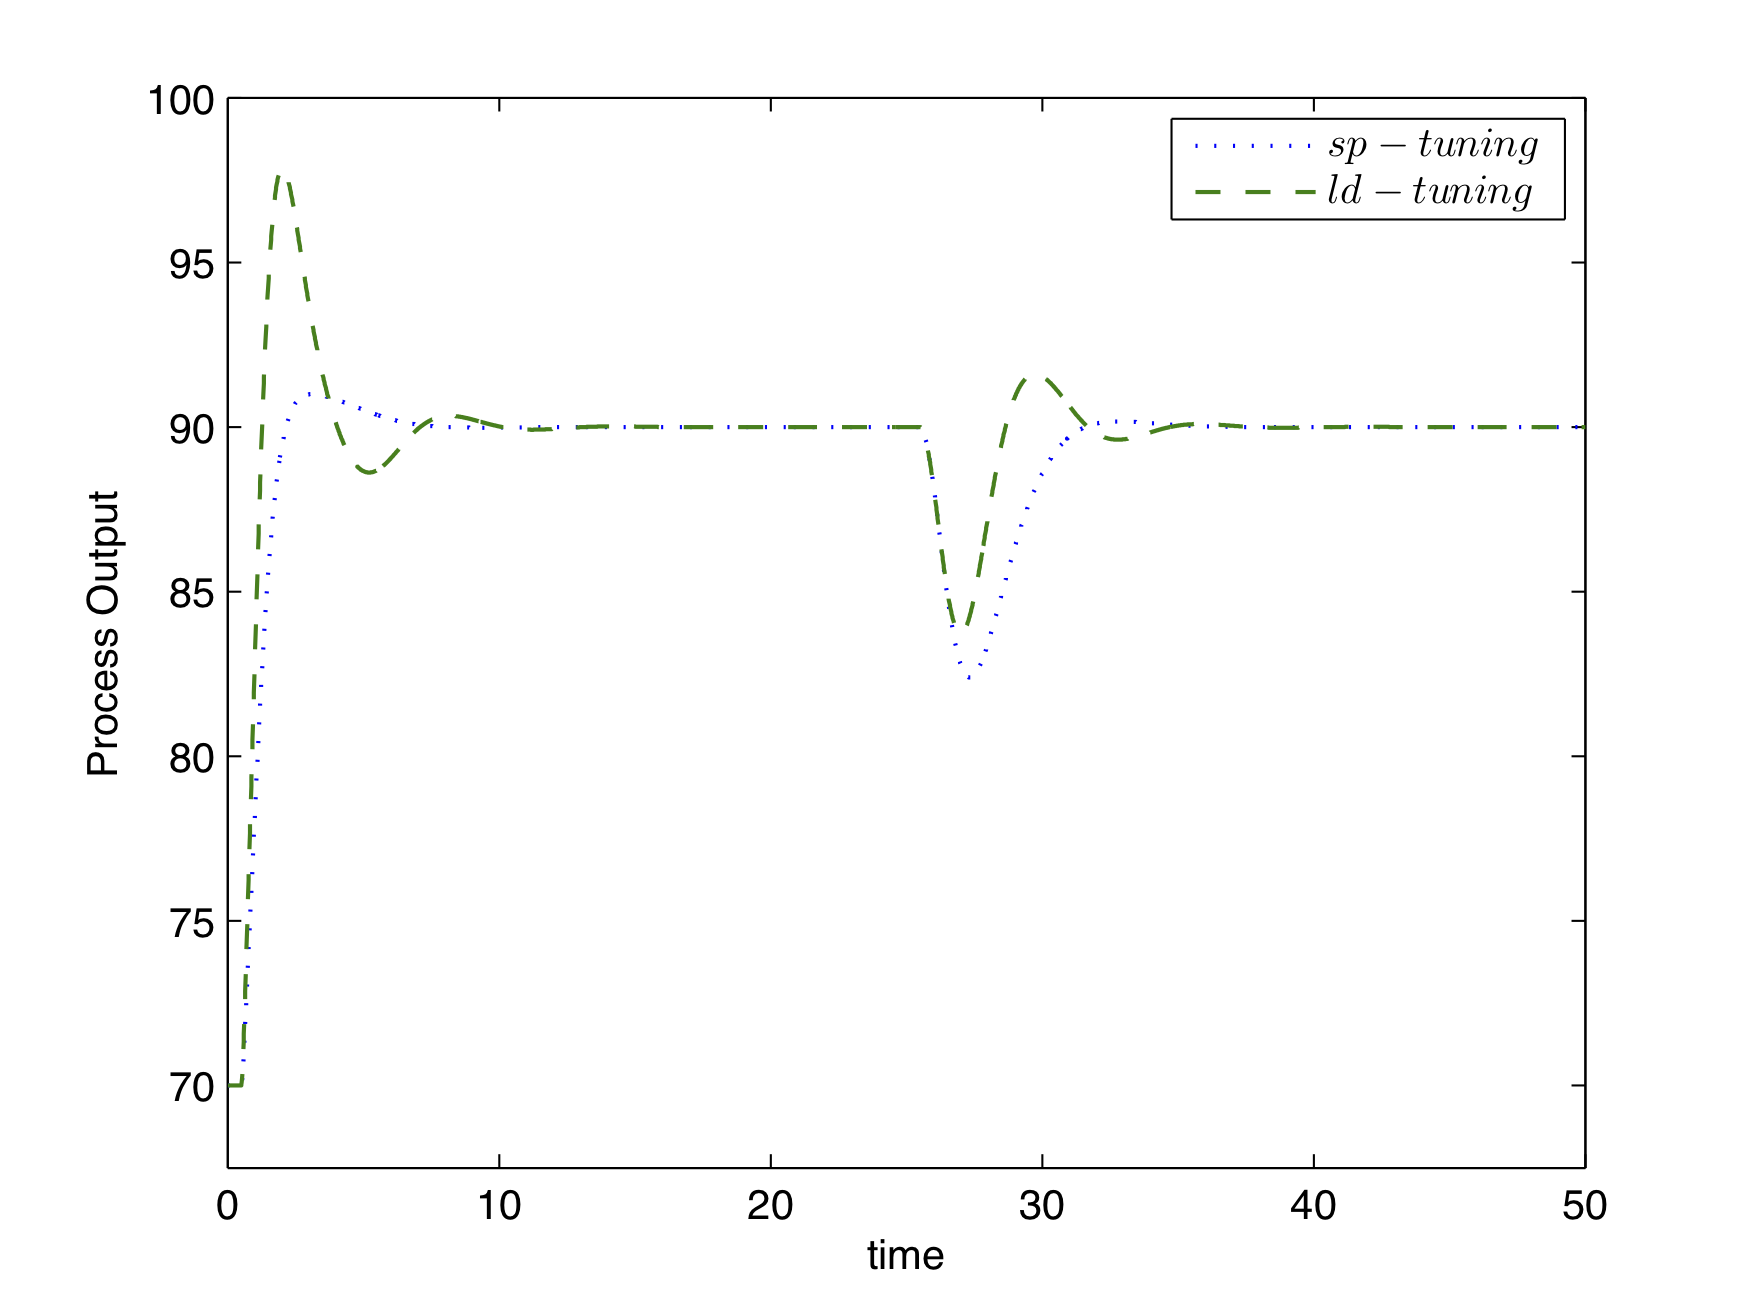
\includegraphics[width=\columnwidth]{Ch3fig22.png}
        \caption{Process responses for servo and regulation for system \ref{system_example}.}
        \label{ch3:fig:example1}
    \end{center}
\end{figure}
%
%
\subsection{Performance vs. Robustness}
%
Robustness is an important attribute for control systems, because the design procedures are usually based on the use of low-order linear models identified at the closed-loop operation point. If only the system performance is taken into account, using by example an integrated error criteria (\gls{iae}, \gls{itae} or \gls{ise}), or a time response characteristic (overshoot, rise-time or settling-time for example), as in \cite{Huang2002, Tavakoli2003}, the resulting closed-loop control system probably will have a very poor robustness.  On the other hand, if the system is designed to have good robustness, as in \cite{Hagglund2008}, and if the performance of the resulting system is not evaluated, the designer will not have any indication of the \emph{cost} of having such highly robust system.  System performance and robustness were take into account in \cite{Shen2002, Tavakoli2005}, optimizing its \gls{iae} or \gls{itae} performance but guarantee only the usually accepted minimum level of robustness ($M_S=2$). Therefore, the design of the closed-loop control system must take into account the system performance to load-disturbance and set-point changes and its robustness to variation of the controlled process characteristics, preserving the well-known \emph{trade-off} between all these variables.

At this point, we can recover the \gls{cstr} reactor example of the previous chapter. In order to illustrate the performance / robustness tradeoff, we consider here the tuning of a \gls{pid} controller in order to achieve different levels of robustness. The MoReRT method from \cite{Alfaro2016}. As the MoReRT allows a desired robustness level to be imposed as a design specification, two cases have been considered here: (a) for $M_S=2.0$ the controller parameters are: $K_p=3.335$, $T_i =0.685 min$, $T_d=0.181 min$, (b) for $M_S=1.6$, the controller parameters are: $K_p=2.372$, $T_i=0.663 min$, $T_d=0.162 min$. As it can be seen, robust designs, corresponding to lower values of $M_S$, correspond lo lower controller gains. As a result, time responses will be smoother but the performance indexes will worsen. Results are shown in table \ref{tab:cstrtradeoff} and figure (\ref{ch3:fig:Ch3FigureClosedLoopRobustnessServoRegulation}). 
%
\begin{figure}[tb]
    \begin{center}
        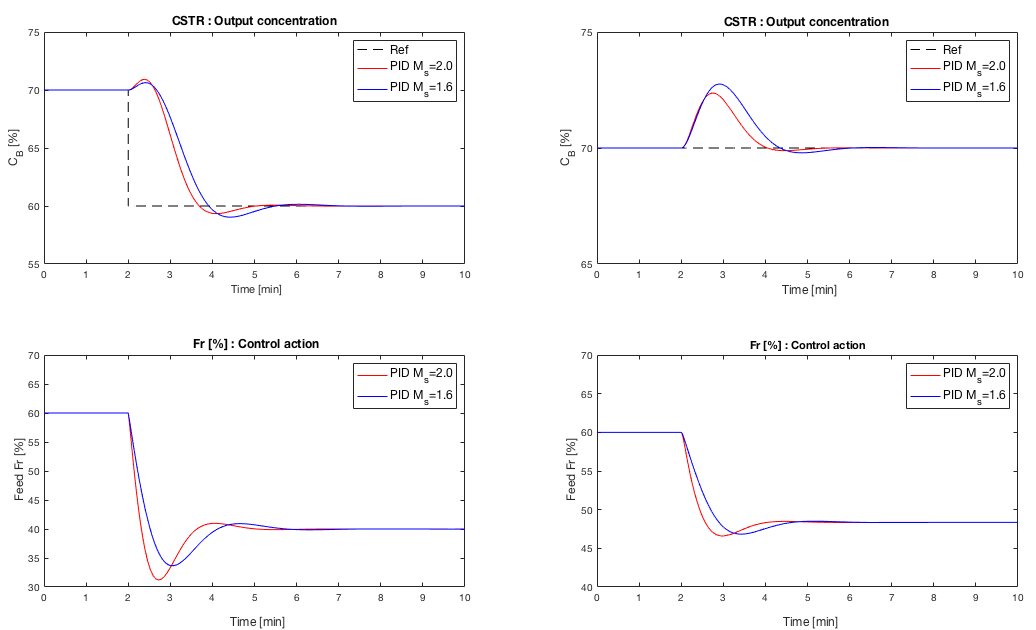
\includegraphics[width=\linewidth]{Ch3FigureClosedLoopRobustnessServoRegulation.png}
        \caption{CSTR reactor time output and control effort to a reference step change and disturbance at the inlet $C_{Ai}$ concentration }
        \label{ch3:fig:Ch3FigureClosedLoopRobustnessServoRegulation}
    \end{center}
\end{figure}

Table \ref{tab:cstrtradeoff} shows the \gls{iae} performance indexes for the output concentration deviations as well as the \gls{tv} for the control effort corresponding to a disturbance change at the input concentration $C_{Ai}$ as well as to a desired change in the operating point, this is the desired output concentration $C_B$. It is seen that the performance is worse for the more robust design but, on the other hand, the control effort gets smoother. 
\begin{table}[tb]
	\caption{Robustness - Performance tradeoff CSTR example} \label{tab:cstrtradeoff}
	\centering
    \begin{tabular}{ccccc}
    \toprule
    	 & \multicolumn{2}{c}{Set-point change for $C_B$}  & \multicolumn{2}{c}{Disturbance at $C_{Ai}$ concentration}\\
   		 & IAE & TV & IAE & TV\\
    \midrule
    $M_s=2.0$ PID Design   & 12.00 & 35.42 & 2.58 & 15.36 \\
    $M_s=1.6$ PID Design   & 14.05 & 34.30 & 3.66 & 13.60 \\
    \bottomrule
    \end{tabular}
\end{table}
%
\subsection{Input vs. Output Disturbances}
%
Disturbance attenuation is often recognised as the primary concern of a control system. Regulation of the operating conditions is the usual task work to be pursued by a feedback controller. However, much of the academic works almost concentrate on set-point experiments for controller evaluation.  Therefore a controller design that emphasizes disturbance rejection rather than set-point tracking is an important design problem that, even if it has been the focus of research it may have not received the appropriate attention. Indeed much of the design approaches as well as application and/or simulation examples provided in academic works almost concentrate on set-point experiments for controller evaluation. Even those that explicitly concentrate on the disturbance attenuation problem, usually concentrate on input load disturbances.

There is however a disturbance attenuation consideration not taken into account, as far as the knowledge of the authors concern. This is that of considering a different load disturbance dynamics path. As mentioned in \cite{Shinskey2002}, there are some processes that exhibit different dynamics in the load path. These include heat exchangers, where the load can enter the tube bundle whereas the manipulated flow enters the shell (or vice versa), and distillation columns, where the load is the feed and the manipulated flow is boil up or reflux.

As a matter of a simple example, the controller used in the previous section, the one with $M_S=2.0$ is faced here to three different disturbances:
%
\begin{itemize}
\item A disturbance that  enters at the process input, a load disturbance. This is exemplified here by a 10\% disturbance at the inlet flow rat $F_r$ 
\item A disturbance that enters at  an intermediate point of the process dynamics.. This is exemplified here by a 10\% disturbance at the inlet concentration of the $A$ component.
\item A disturbance that affects directly at the process output. This is exemplified here by a 10\% disturbance at the output concentration of the $B$ component. $C_B$
 \end{itemize} 

As it can be seen in figure (\ref{ch3:fig:Ch3FigureClosedLoopDisturbances}), even the size of the disturbance is the same in all three situations, the response of the controller is different. In case of the output disturbance, its dynamics is commonly associated to the one for a reference change. In fact, the disturbance signal enters at the same point in the block diagram (except for eventual sensor measurement noise). Therefore, depending on the control system specifications, the attenuation of one disturbance or the other requires different considerations. Adding, in addition to the other two tradeoffs just presented above, a third potential source of conflicting objectives that motivates the need for a multiobjective approach.
%
\begin{figure}[tb]
    \begin{center}
        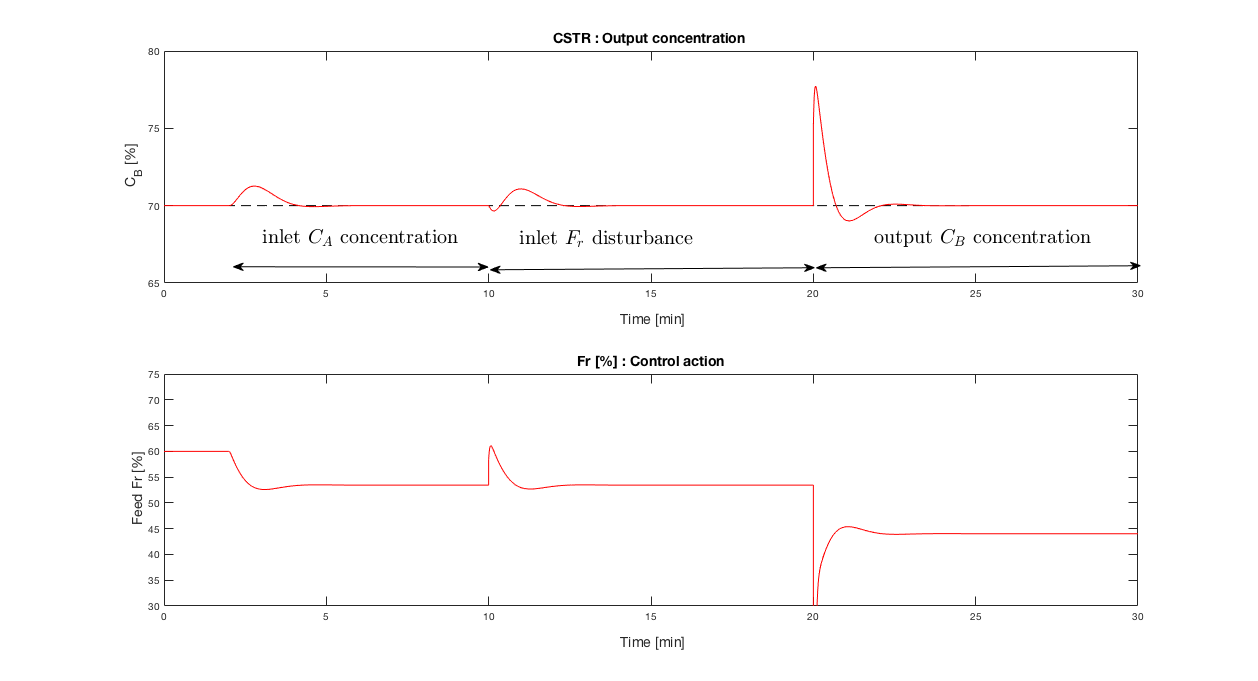
\includegraphics[width=\columnwidth]{Ch3FigureClosedLoopDisturbances.png}
        \caption{CSTR output $C_B$ concentration in response to different disturbances.}
        \label{ch3:fig:Ch3FigureClosedLoopDisturbances}
    \end{center}
\end{figure}
%
\bibliographystyle{spbasic}
\bibliography{ReferenciasMulti}